\chapter{Realizacja projektu}
%______________________________________________________________________________________________________________
\newcolumntype{C}[1]{>{\centering}m{#1}}

Niniejszy rozdział zawiera opis przebiegu realizacji projektu. Pokrótce zaprezentowano narzędzia programistyczne wykorzystane w trakcie prac na projektem. Przedstawiono wykaz podzespołów wraz z krótką charakterystyką, szczegóły dotyczące modyfikacji przerzutki, integracji elementów elektronicznych oraz implementacji głównych funkcjonalności sterownika.
   
\section{Narzędzia programistyczne}
Komputer klasy PC stanowi podstawę środowiska do rozwoju aplikacji na wybraną platformę sprzętową oraz do przeprowadzania testów wykonanego układu.
 
Program sterownika został napisany w języku C, który jest powszechnie wykorzystywany w aplikacjach wbudowanych. Język opracowany przez Dennisa Ritchego, w latach siedemdziesiątych ubiegłego wieku w Bell Laboratories \cite{prata}. Doskonale nadaje się do aplikacji niskopoziomowych ze względu na łatwą przenośność kodu, elastyczność oraz wysoką wydajność aplikacji napisanych w tym języku. 
\subsection{Code Composer Studio 6.0.0}

Oprogramowanie sterownika rozwijane było w oparciu o zintegrowane środowisko programistyczne Code Composer Studio v6.0.0 oferowane przez Texas Instruments. Środowisko umożliwia wykonanie aplikacji na różne platformy sprzętowe TI. Są to m.in. mikrokontrolery z serii Tiva/Stellaris, procesory sygnałowe z rodziny TMS320 czy układy SOC (ang. {\em System On Chip}) serii DaVinci. CCS v6.0.0 łączy zalety środowiska Eclipse Kepler 4.3, które stanowi bazę CCS, z narzędziami do rozwijania aplikacji embedded, takimi jak kompilator ARM GNU Linaro, czy wbudowany debugger.
%______________________________________________________________________________________________________________
\subsection{Biblioteka \textit{TivaWare Peripheral Driver}}
Texas Intrusments dostarcza bibliotekę dedykowaną do mikrokontrolerów z rodziny Tiva ARM Cortex-M - \textit{TivaWare  Peripheral Driver Library}. Biblioteka stanowi zbiór funkcji umożliwiających wykorzystanie układów peryferyjnych mikrokontrolera. Biblioteka, napisana w języku C, wspiera dwa modele programowania mikrokontrolera - Direct Register Access oraz Software Driver Model. Pierwszy z nich operuje bezpośrednio na rejestrach mikrokontrolera, co pozwala pisać bardzo wydajne programy o niewielkim rozmiarze. Jednocześnie wymaga bardzo dobrej znajomości rejestrów mikrokontrolera, znaczenia poszczególnych bitów oraz zależności pomiędzy rejestrami. Software Driver Model działa na wyższym poziomie dając kontrolę nad całymi układami peryferyjnymi. Użytkownik nie musi znać dokładnej architektury mikrokontrolera, co znacząco przyspiesza proces rozwijania oprogramowania. 
%______________________________________________________________________________________________________________
\subsection{Pozostałe oprogramowanie}
Pozostałe oprogramowanie wykorzystane w trakcie realizacji projektu to m.in.:
\begin{itemize}
\item
Saleae Logic - oprogramowanie współpracujące z analizatorem stanów logicznych,
\item
Gnuplot - program do graficznej reprezentacji danych,
\item
Putty - klient usług Telnet, SSH i rlogin, wykorzystany do logowania danych,
\item
Eagle - program do projektowania układów elektronicznych,
\item
FreeCad - program do modelowania parametrycznego 3D,
\item
QT Creator - środowisko do projektowania interfejsu graficznego z wykorzystaniem biblioteki QT.
\end{itemize}
%______________________________________________________________________________________________________________
\section{Wykaz podzespołów}
\subsection{Przerzutka tylna}
Autor zdecydował się na wykorzystanie tylnej przerzutki SRAM X5 \cite{sramX5}. Głównym atutem tej przerzutki jest jej konstrukcja, która ze względu na długie ramiona wózka przerzutki, umożliwia bezproblemowe zamontowanie serwomechanizmu. Przerzutka oferuje pełny zakres ruchu do obsługi ośmiu przełożeń. Dodatkowo jest solidną propozycją z niskiej półki cenowej.
%_______________________________________________________________________________________________________________
\subsection{Serwomechanizm}
Serwomechanizm odpowiedzialny za pozycjonowanie wózka przerzutki to Hitec Hs-8335SH. Jest to tzw. cyfrowy serwomechanizm, przeznaczony do zastosowań modelarskich. Od analogowych odpowiedników odróżnia się większą precyzją w osiąganiu zadanej pozycji oraz wyższym momentem obrotowym. Autor zdecydował się na zastosowanie gotowego serwomechanizmu z kilku powodów. Takie rozwiązanie zdecydowanie przyspieszyło prace nad projektem. W dodatku gotowy serwomechanizm charakteryzuje się kompaktowymi rozmiarami oraz odpornością na warunki atmosferyczne.  

Parametry techniczne serwomechanizmu Hitec Hs-8335SH:
\begin{itemize}
\item
Napięcie robocze [V]: 6-7.4,
\item
Moment obrotowy (7.4V)[kgcm]: 24,
\item
Prędkość (7.4V)[sek/$60^{\circ}$]: 0.13,
\item
Metalowe tryby przekładni.
\end{itemize} 
\label{serwo}
%_______________________________________________________________________________________________________________
\subsection{Mikrokontroler}
Sterownik nadzorujący pracę całego układu został wykonany w oparciu o zestaw uruchomieniowy Texas Instruments Tiva C-Series EK-TM4C123GXL. Zestaw zawiera 32-bitowy mikrokontroler TM4C123GH6PM wykorzystujący rdzeń ARM Cortex-M4F \cite{tiva}. Posiada wbudowany regulator 3.3V, port micro USB oraz wyprowadzenia niezbędnych portów I/O. Charakteryzuje się kompaktowymi rozmiarami. Mikrokontroler zastosowany w zestawie 	oferuje wysoką wydajność oraz niski pobór prądu. Kontroler przerwań sprzętowych NVIC (ang. {\em Nested Vectored Interrupt Controller}) umożliwia efektywne zarządzanie przerwaniami w zależności od zaprogramowanych priorytetów \cite{tiva}.

Parametry techniczne mikrokontrolera:
\begin{itemize}
\item
Zegar systemowy taktowany z częstotliwością do 80 MHz,
\item
Rdzeń ARM Cortex-M4F,
\item 
Obsługuje zestaw instrukcji Thumb2,
\item
Pamięć flash 256kB,
\item
Pamięć SRAM 32kB,
\item
43 porty I/O,
\item
Generator sygnału PWM,
\item
Kontroler DMA,
\item
Kontroler transmisji szeregowej(USB 2.0, UART, I2C, SPI, CAN),
\item
Układy czasowo-licznikowe.
\end{itemize} 
%_______________________________________________________________________________________________________________
\subsection{Czujniki pomiarowe}
%_______________________________________________________________________________________________________________
\subsubsection{Pololu AltIMU 10}

Pololu AltIMU10 to inercyjna jednoskta pomiarowa, w skład której wchodzą czujniki wykonane w technologii MEMS:
\begin{itemize}
\item
trzyosiowy akcelerometr ST LSM303DLHC,
\item
trzyosiowy żyroskop ST L3GD20,
\item
trzyosiowy magnetometr ST LSM303DLHC.
\end{itemize}

Wszystkie czujniki zamontowane w jednostce komunikują się z urządzeniem nadrzędnym z wykorzystaniem magistrali I2C (ang. {\em Inter-Intergrated Circuit}). Magistrala I2C jest szeregowym, dwukierunkowym interfejsem komunikacyjnym opracowanym przez firmę Philips. Układ AltImu10 posiada elementy pasywne, gwarantujące poprawne działanie magistrali, oraz wbudowany regulator napięcia \cite{Pololu}.
%______________________________________________________________________________________________________________
\subsubsection{Zbliżeniowe czujniki magnetyczne}
Zbliżenie czujniki załączane magnetycznie, o oznaczeniu CMD14, wykorzystane są do wyznaczania prędkości obrotowych tylnego koła oraz mechanizmu korbowego. W wyniki działania pola magnetycznego, pochodzącego z magnesu trwałego, czujnik zwiera swoje styki. 
 
Parametry techniczne:
\begin{itemize}
\item
Maksymalne napięcie pracy [V] : 50,
\item
Maksymalny prąd [A]: 0.1,
\item
Maksymalny zasięg [mm]: 25,
\item
Styk normalnie otwarty.
\end{itemize}
%_______________________________________________________________________________________________________________
\subsection{Układ zasilania}
Źródłem zasilania całego układu jest pakiet litowo-polimerowy BRAINERGY 1000mAh.
Parametry techniczne pakietu zasilającego:
\begin{itemize}
\item
Pojemność [mAh]: 1000,
\item
Liczba ogniw: 2,
\item
Napięcie robocze [V]: 7.4,
\item
Wydajność prądowa [A]: 45.
\end{itemize}

Dodatkowo zastosowany został regulator napięcia obniżający wartość napięcia pakietu do 5V, które jest źródłem zasilania zestawu uruchomieniowego EK-TM4C123GXL.
%______________________________________________________________________________________________________________



\section{Modyfikacja przerzutki}
 Zasada działania serwomechanizmu kontrolującego pozycję wózka została przedstawiona na rys. \ref{fig:przerzutkaSerwo}. Zmiana pozycji wału serwomechanizmu implikuje zmianę pozycji wózka poprzez zastosowanie sztywnego połączenia przegubowego.
 \begin{figure}[h]
    \centering
    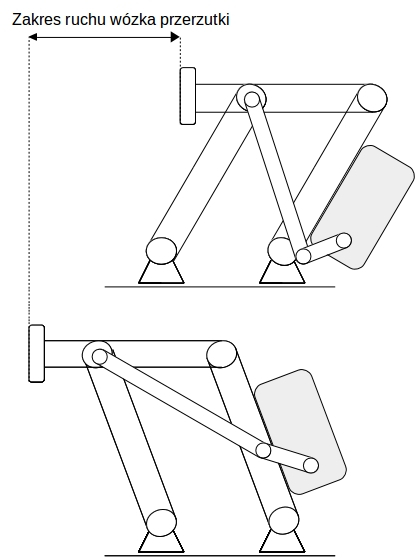
\includegraphics[scale=0.4]{przerzutkaSerwo.jpg}
    \caption{Zasada działania przerzutki rowerowej z wykorzystaniem serwomechanizmu.}
    \label{fig:przerzutkaSerwo}
\end{figure}

\begin{figure}[h]
    \centering
    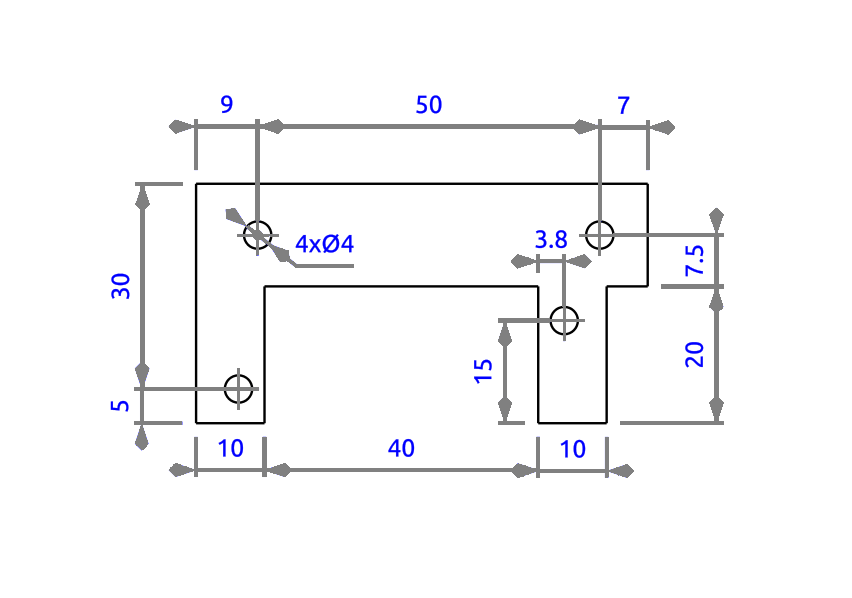
\includegraphics[scale=0.3]{lacznik.png}
    \caption{Rysunek techniczny elementu mocującego serwomechanizm do przerzutki.}
    \label{fig:lacznik}
\end{figure}

Przymocowanie serwomechanizmu do przerzutki, zgodnie ze schematem przedstawionym na rys. \ref{fig:przerzutkaSerwo}  można podzielić na kilka etapów.
Pierwszy etap to usunięcie sprężyny, która występuje w konwencjonalnych przerzutkach tylnych. Wiąże się to ze zniszczeniem połączeń nitowych do których przymocowana jest sprężyna. Zniszczone połączenia nitowe zastąpione zostały przez połączenia śrubowe. Wykorzystane zostały śruby z gwintem metrycznym M4 o średnicy 4 mm.

Następny etap to wykonanie elementu mocującego serwomechanizm do przerzutki. Element został wykonany zgodnie z projektem przedstawionym na rysunku technicznym \ref{fig:lacznik}.


Wykonany element wraz z połączeniami śrubowymi umożliwia przymocowanie serwomechanizmu Hitec Hs-8335SH do przerzutki SRAM X5. Ostatni etap tej części projektu to wykonanie połączenia przegubowego łączącego wał serwomechanizmu z jednym z członów ruchomych przerzutki. Autor zdecydował się na zastosowanie modelarskiego drążka kierowniczego o zmiennej długości oraz dedykowanego aluminiowego orczyka serwomechanizmu. Takie rozwiązanie pozwala dokładnie dopasować długość  połączenia, bez konieczności projektowania oraz wykonania dodatkowych elementów.

W wyniku powyższych czynności powstała w pełni funkcjonalna przerzutka tylna sterowana przy użyciu serwomechanizmu. 

%_______________________________________________________________________________________________________________
\section{Integracja elementów elektronicznych}
Mikrokontroler, filtry RC, pakiet zasilający, regulator napięcia oraz jednostka pomiarowa IMU zamontowane zostały w hermetycznej puszcze elektrycznej, przymocowanej na stałe do dolnej rury przedniego trójkąta ramy rowerowej.

\begin{figure}[h]
    \centering
    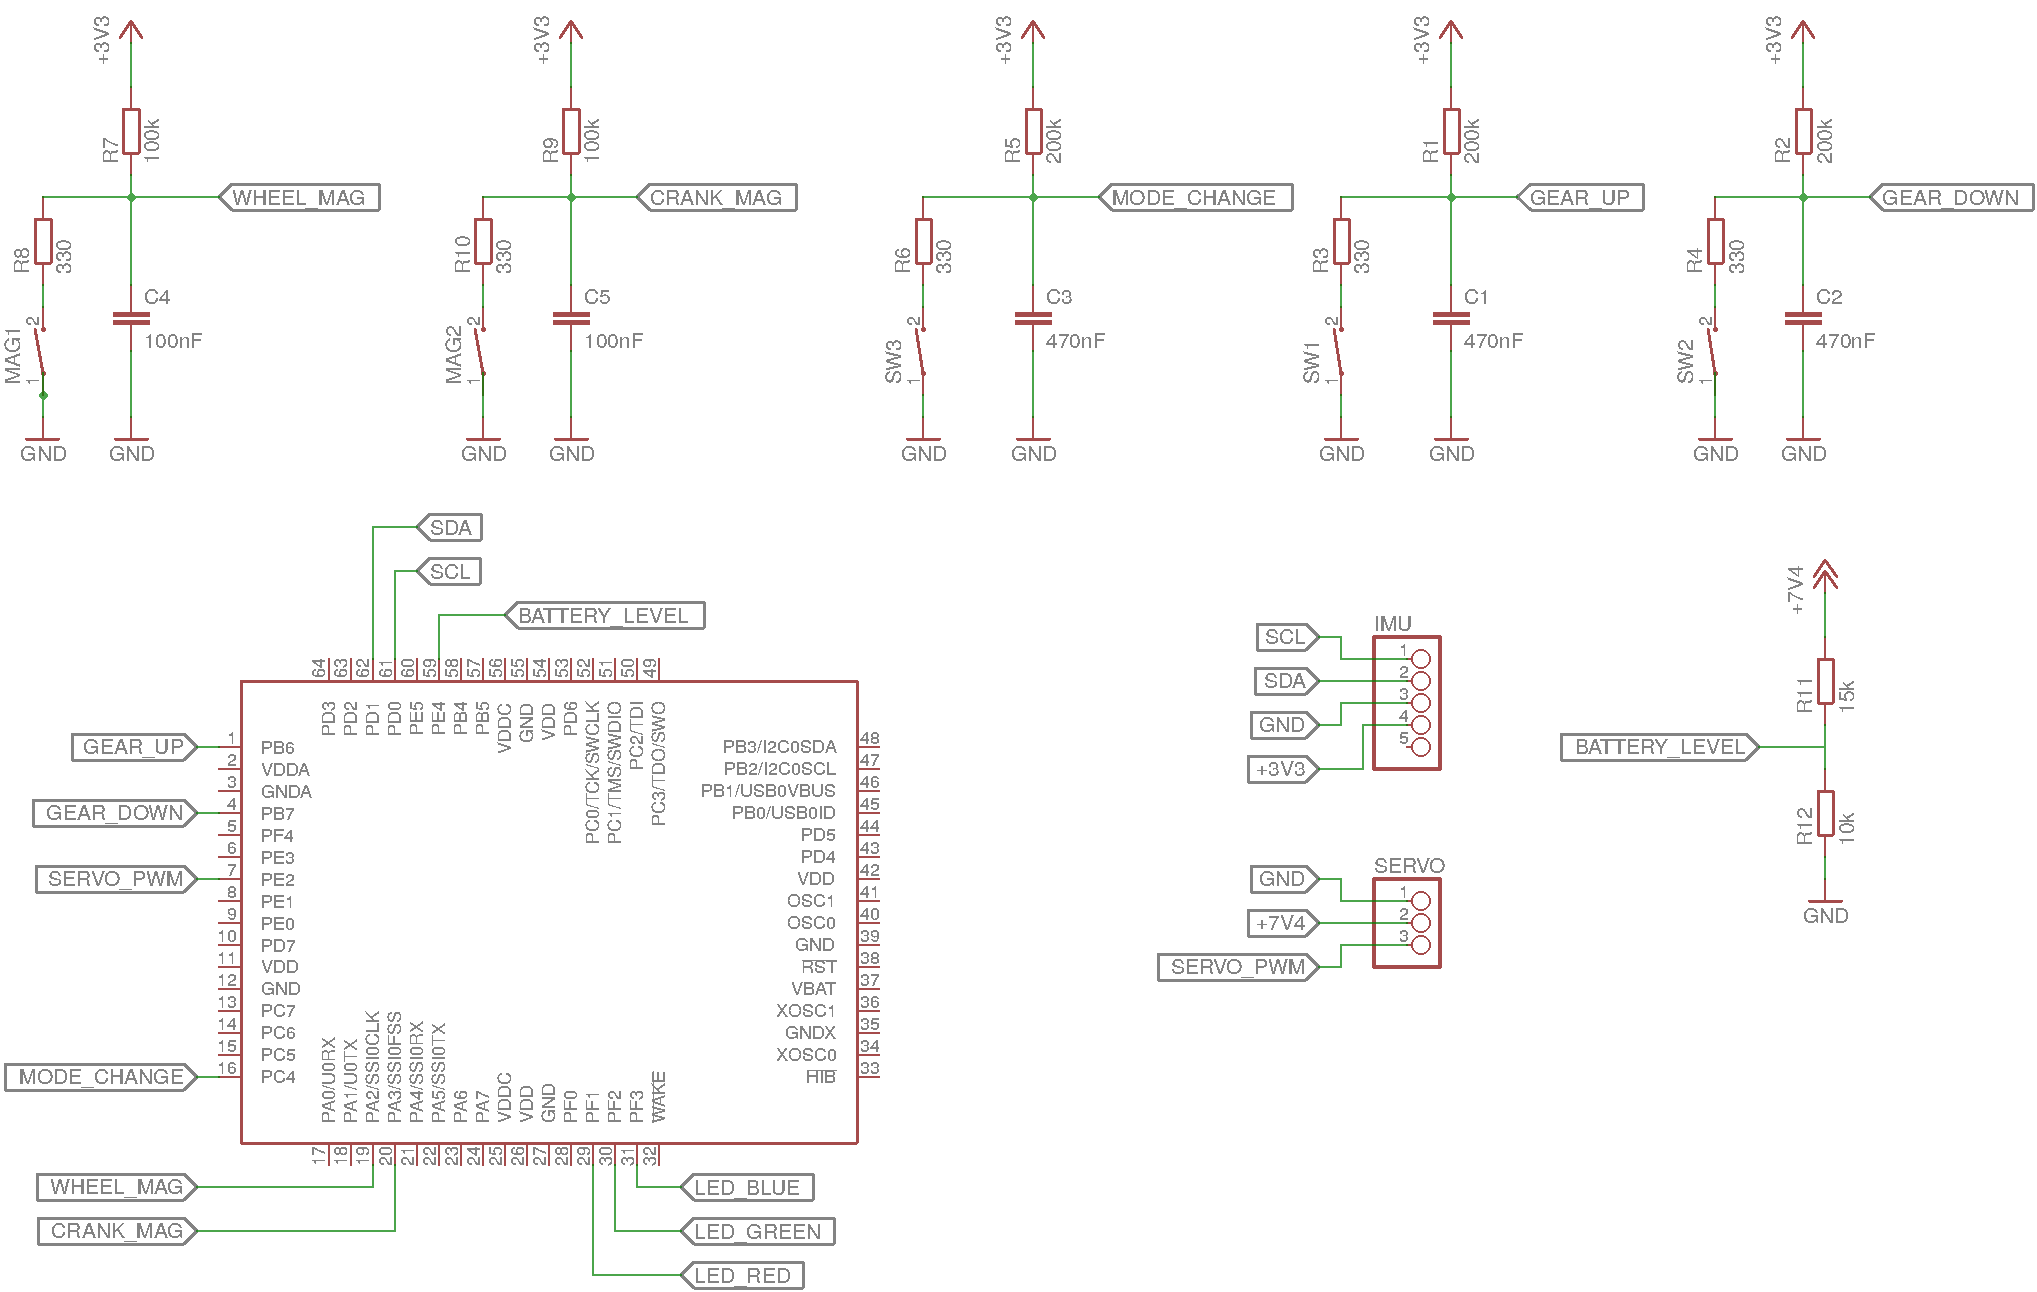
\includegraphics[scale=0.7]{connectionSchematic.png}
    \caption{Schemat połączeń elementów elektronicznych.}
    \label{fig:schematPolaczen}
\end{figure}

\begin{table}[h]
    \caption{Funkcje portów I/O przedstawionych na schemacie połączeń elementów elektronicznych:}
    \begin{center}
		\label{tab:portyGPIO}
		\begin{tabular}{|c|>{\centering}m{8cm}|}
 			\hline
 			\textbf{Nazwa syngału} & \textbf{Funkcja} \tabularnewline
 			\hline
 			GEAR\_UP & Obsługa przycisku zwiększającego przełożenie \tabularnewline
 			\hline
 			GEAR\_DOWN &  Obsługa przycisku zmniejszającego przełożenie \tabularnewline
 			\hline
 			SERVO\_PWM & Generowanie sygnału sterującego pozycją serwomechanizmu \tabularnewline
 			\hline
 			MODE\_CHANGE &  Obsługa przycisku zmiany trybu pracy sterownika\tabularnewline
 			\hline
 			WHEEL\_MAG & Obsługa czujnika magnetycznego do pomiaru prędkości kątowej koła roweru \tabularnewline
 			\hline
 			CRANK\_MAG & Obsługa czujnika magnetycznego do pomiaru kadencji \tabularnewline
 			\hline
 			BATTERY\_LEVEL & Odczyt pomiaru poziomu napięcia \tabularnewline
 			\hline
 			SCL &  Obsługa linii zegarowej magistrali I2C \tabularnewline
 			\hline
 			SDA & Obsługa linii danych magistrali I2C \tabularnewline
 			\hline
		\end{tabular}
	\end{center}
\end{table}

Schemat połączeń znajduje się na rys. \ref{fig:schematPolaczen}. Na schemacie przedstawione zostały jedynie elementy wykonane przez Autora pracy. Są to filtry RC, dzielnik napięcia do pomiaru stanu pakietu zasilającego, połączenia do sterowania serwomechanizmem oraz połączenia do komunikacji z jednostką pomiarową IMU. Szczegóły związane z dystrybucją zasilania zostały pominięte, ponieważ są elementem zestawu uruchomieniowego. Można je znaleźć w dokumentacji urządzenia \cite{tivaWork}. Ze względu na rozwojowy charakter projektu oraz częste zmiany wprowadzane na etapie realizacji, autor pracy nie zdecydował się na wykonanie dedykowanego obwodu drukowanego.
%______________________________________________________________________________________________________________

\section{Implementacja głównych funkcjonalności}
%______________________________________________________________________________________________________________
\subsection{Kontrola serwomechanizmu}
Pozycja serwomechanizmu modelarskiego sterowana jest przez sygnał PWM (ang. {\em Pulse-Width Modulation}). Jest to metoda regulacji sygnałem napięciowym, o stałej częstotliwości i amplitudzie, polegająca na zmianie wypełnienia sygnału. Częstotliwość sygnału wynosi 50Hz. Wartości napięcia, które zmieniają się w sposób skokowy, wynoszą 0 i 3.3V. Pełny zakres ruchu serwomechanizmu osiągalny jest przez zmianę wypełnienia sygnału sterującego z zakresu od 2.5 do 12.5 \%. Innymi słowy - podanie prostokątnego sygnału sterującego o okresie 20ms, w którym stan wysoki utrzymany jest przez czas z zakresu od 0.5ms do 2.5 ms, umożliwia obrót wału serwomechanizmu z zakresu od 0 do 180$^{\circ}$.

Przerzutka, do której został przymocowany serwomechanizm, ogranicza pełny zakres ruchu serwomechanizmu. Minimalne oraz maksymalne wychylenie wózka przerzutki wiąże się z obrotem wału serwomechanizmu odpowiednio o kąt 31 i 95$^{\circ}$. W tym zakresie obsługiwane są wszystkie dostępne przełożenia. Każdemu z ośmiu przełożeń odpowiada inna pozycja serwomechanizmu (tabela \ref{tab:przelozenia}). Pozycje serwomechanizmu zostały dobrane eksperymentalnie. Można zaobserwować liniowy przyrost czasu wypełnienia sygnału. 

\begin{table}[h]
    \caption{Pozycja serwomechanizmu oraz czas wypełnienia sygnału PWM w zależności od aktualnego przełożenia:}
    \begin{center}
		\label{tab:przelozenia}
		\begin{tabular}{|>{\centering}m{2cm}|>{\centering}m{3cm}|>{\centering}m{4cm}|}
			\hline
 			\textbf{Nr przełożenia} & \textbf{Pozycja serwomechanizmu [$^{\circ}$]} & \textbf{Czas wypełnienia sygnału [$us$]} \tabularnewline 
 			\hline
 			1 & 31.5 & 850 \tabularnewline 
 			\hline 
			2 & 40.5 & 950 \tabularnewline 
			\hline
			3 & 49.5 & 1050 \tabularnewline  
			\hline
			4 & 58.5 & 1150 \tabularnewline  
			\hline
			5 & 67.5 & 1250 \tabularnewline  
			\hline
			6 & 76.5 & 1350 \tabularnewline  
			\hline
			7 & 85.5 & 1450 \tabularnewline  
			\hline
			8 & 94.5 & 1550 \tabularnewline 
			\hline
		\end{tabular}
	\end{center}
\end{table}

Z doświadczenia autora pracy wynika, że zmiana przełożeń w konwencjonalnych układach napędowych działa znacznie lepiej, jeśli w trakcie zmiany biegu następuje chwilowe przeciągnięcie pozycji wózka przerzutki. Jest to szczególnie dobrze widoczne w trakcie redukowania przełożenia, kiedy łańcuch powinien trafić na koło zębate o większej średnicy. Można wtedy zaobserwować opóźnienie w zmianie przełożenia, niekorzystne przeskoki łańcucha pomiędzy kołami zębatymi, a w źle wyregulowanych układach napędowych może nawet dochodzić do braku reakcji układu napędowego. Takie zjawisko zostało zaobserwowane w trakcie pracy nad projektem. Zmiana biegów polegająca na pozycjonowaniu serwomechanizmu w nowej pozycji, zależnej od dobranego przełożenia, działała z wyraźnym opóźnieniem. Problem, podobnie jak w układach mechanicznych, został rozwiązany przez chwilowe przeciągnięcie pozycji wózka przerzutki. Zdefiniowanie zostały dwa pomocnicze zestawy pozycji serwomechanizmu, specyficzne dla redukowania oraz zwiększania przełożenia (tabela \ref{tab:przelozeniaPomocniczne}). Wszystkie trzy zestawy pozycji przechowywane są w postaci tablic, które zawierają czasy wypełnienia sygnału sterującego. W momencie rozpoczęcia zmiany przełożenia, na skutek naciśnięcia przycisku lub w wyniku decyzji kontrolera automatycznej zmiany przełożeń, zmienna, która do tej pory wskazywała na główny zestaw pozycji, zaczyna wskazywać na jeden z zestawów pomocniczych zależny od rodzaju zmiany. Jednocześnie uruchomiony zostaje układ czasowo-licznikowy. Po upływie 500ms, w trakcie obsługi przerwania tego układu, następuje przypisanie adresu, pod którym znajduje się w pamięci główny zestaw parametrów. Następuje również wyłączenie układu czasowo-licznikowego. 


\begin{table}[h]
    \caption{Pomocnicze zestawy pozycji serwomechanizmu:}
    \begin{center}
		\label{tab:przelozeniaPomocniczne}
		\begin{tabular}{|>{\centering}m{2cm}|>{\centering}m{4cm}|>{\centering}m{4cm}|}
			\hline
 			\textbf{Nr przełożenia} & \textbf{Wypełnienie sygnału w trakcie redukcji przełożenia} [$us$] & 
\textbf{Wypełnienie sygnału w trakcie zwiększenia przełożenia [$us$]} \tabularnewline
 			\hline
 			1 & 800 & 900 \tabularnewline
 			\hline
			2 & 900 & 1000 \tabularnewline
			\hline
			3 & 1000 & 1100 \tabularnewline  
			\hline
			4 & 1100 & 1200 \tabularnewline  
			\hline
			5 & 1200 & 1300 \tabularnewline  
			\hline
			6 & 1300 & 1400 \tabularnewline  
			\hline
			7 & 1400 & 1500 \tabularnewline  
			\hline
			8 & 1500 & 1600 \tabularnewline 
			\hline
		\end{tabular}
	\end{center}
\end{table}
%______________________________________________________________________________________________________________
\subsection{Obsługa przycisków}
W projekcie wykorzystane zostały trzy przyciski przewlekane, monostabilne. Ich naciśnięcie powoduje redukcję lub zwiększenie przełożenia oraz zmianę trybu pracy kontrolera. Przyciski do zmiany przełożenia zamontowane zostały w miejscu konwencjonalnej manetki. Przycisk do zmiany trybu pracy został przymocowany do mostka kierownicy.

Wszystkie przyciski wykorzystują rezystor pull-up, podciągający do portu wejściowego napięcie 3.3V (rys. \ref{fig:schematPolaczen}). Zwarcie przycisku powoduje ustalenie sygnału na poziomie 0V. Pojawienie się na magistrali zbocza opadającego powoduje zgłoszenie przerwania od odpowiedniego pinu portu wejściowego. 

Z przyciskami związany jest problem drgań styków w trakcie zwierania/rozwierania przycisku. Są to drgania mechaniczne, które mogą trwać od kilku mikrosekund do nawet kilkunastu milisekund. Powoduje to niezdefiniowane zachowanie całego systemu, np. zmianę kilku przełożeń na raz. Szybkozmienne zmiany stanu logicznego sygnału, wynikające z drgań styków przycisku, przedstawione zostały na rys \ref{fig:drganiaPrzyciskow}.
\begin{figure}[h]
    \centering
    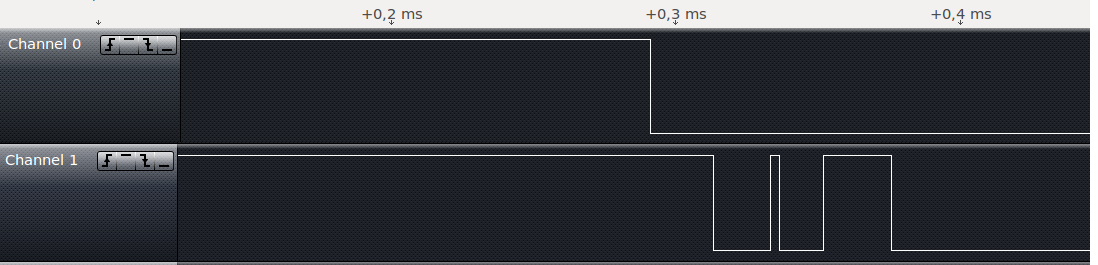
\includegraphics[scale=0.35]{drganiaPrzyciskow.png}
    \caption{Porównanie przebiegów sygnałów interpretowanych przez analizator stanów logicznych dla przycisku z filtrem RC - kanał 0, oraz bez filtra- kanał 1.}
    \label{fig:drganiaPrzyciskow}
\end{figure}
Istnieje kilka sposobów rozwiązania tego problemu. Można je podzielić na sposoby programowe oraz sprzętowe. Sposoby programowe to np. kilkukrotne sprawdzenie stanu portu wejściowego lub chwilowe wyłączenie przerwań od portów wejściowych. Autor zdecydował, że lepszym rozwiązaniem będzie usunięcie przyczyny tego zjawiska, czyli odpowiednie kondycjonowanie sygnału. W tym celu wykonane zostały proste filtry dolnoprzepustowe RC. Zasada działania filtru RC została opisana w pkt. \ref{filtrRc}. W dokumentacji mikrokontrolera można znaleźć informację na temat minimalnego poziomu napięcia, interpretowanego jako stan wysoki - $0.6V_{in}$ \cite{tiva}. Podobny poziom napięcia osiągany jest na wyjściu filtru RC, po skokowej zmianie napięcia wejściowego, po czasie równym stałej czasowej filtra. Autor założył, że zmiany biegów, oraz zmiana tryb jazdy, nie mogą być dokonywane częściej, niż 10 razy na sekundę. Z tego wynika, że stała czasowa filtru powinna wynosić około $100ms$. Wszystkie 3 filtry zostały wykonane z użyciem opornika o rezystancji $200k\Omega$ i kondensatoa o pojemności 470$nF$. Tak dobór elementów pasywnych pozwala zbudować filtr, którego stała czasowa wynosi około $94ms$.
%______________________________________________________________________________________________________________
\subsection{Obsługa zbliżeniowych czujników magnetycznych}
Zbliżeniowe czujniki magnetyczne działają w sposób analogiczny do przycisków monostablilnych. Różnica polega na tym, że styki zwierane są w wyniku działania zewnętrznego pola magnetycznego, pochodzącego od magnesu trwałego. W trakcie zwierania/rozwierania czujnika magnetycznego również pojawia się problem mechanicznych drgań styków. Problem został wyeliminowany w taki sam sposób, jak w przypadku przycisków - przez zastosowanie filtrów dolnoprzepustowych RC. Elementy pasywne filtrów RC Stałe dla czujników magnetycznych zostały dobrane zgodnie z poniższymi założeniami.

Czujnik magnetyczny, wykorzystany do wyznaczania chwilowej wartości prędkości roweru, korzysta z dwóch magnesów trwałych. Doświadczenia przeprowadzone z wykorzystaniem analizatora stanów logicznych przy dużych prędkościach obrotowych tylego koła wykazały, że drgania czujników magnetycznych trwają nie dłużej niż 1ms.  Autor założył, że maksymalna prędkość roweru możliwa do osiągnięcia to 100$\frac{km}{h}$, czyli około 28$\frac{m}{s}$. Promień koła roweru wynosi około 0.33m. Z zależności (\ref{eq:zaleznoscNaPredkosc}) wynika, że dla prędkości maksymalnej, magnes trwały znajduje się w pobliżu czujnika magnetycznego co 37ms. Należy uwzględnić również to, że w tym czasie dochodzi do zwarcia i rozwarcia czujnika magnetycznego. Stała czasowa filtru RC, powinna być zatem co najmniej dwa razy krótsza. Ostatecznie filtr RC został wykonany z opornika o rezystancji 100k$\Omega$ i kondensatora o pojemności 100nF, co zapewnia wartość stałej czasowej filtra na poziomie 10ms. Wartość ta jest o rząd wielkości większa od zarejestrowanych okresów drgań, a jednocześnie zwarcie i rozwarcie czujnika z filtrem trwa prawie dwa razy krócej, niż okres obrotu magnesu trwałego dla przyjętej prędkości maksymalnej.

Czujnik magnetyczny wykorzystywany do wyznaczenia chwilowej wartości kadencji jest zwierany przez jeden magnes trwały, przymocowany do ramienia mechanizmu korbowego. Autor przyjął, że maksymalna kadencja możliwa do osiągnięcia przez rowerzystę, to 250$\frac{obr}{min}$. Pełny obrót przy takie kadencji zajmuje 240ms. Zastosowanie filtru o takiej samej stałej czasowej, jak filtr czujnika magnetycznego prędkości roweru, spełnia wymagania wynikające z przyjętego założenia o maksymalnej kadencji. 
%______________________________________________________________________________________________________________
\subsection{Obsługa jednostki pomiarowej Pololu AltIMU10}
Dane pomiarowe pochodzące z akcelerometru oraz żyroskopu wykorzystywane są w trybie active i sport. Kąt nachylenia podłoża wyznaczany jest co 10ms przy użyciu filtru komplementarnego, którego zasadę działania opisano w pkt. \ref{kompZasadaDzialania}. 
 
Komunikacja pomiędzy mikrokontrolerem a jednostką pomiarową zachodzi przy użyciu magistrali I2C. Magistrala działa w tybie \textit{standard mode}, w którym prędkość transmisji danych wynosi 100$kb/s$. Jednostka pomiarowa posiada pięć wyprowadzeń wyjściowych, jednak w projekcie używane są tylko cztery:
\begin{itemize}
    \item
    SCL (ang. {\em Serial Clock Line}) - linia zegarowa wykorzystana do synchronizacji transferu danych,
    \item
    SDA (ang. {\em Serial Data Line}) - linia danych wykorzystana do przesyłu danych,
    \item
    Vin - zasilanie jednostki pomiarowej, które przyjmuje napięcie z zakresu od 2.5V do 5.5V,
    \item
    GND - wspólna masa.
\end{itemize} 

Komunikacja w standardzie I2C jest komunikacją typu master/slave. Urządzeniem nadrzędnym, odpowiedzialnym za inicjowanie, prowadzenie oraz kontrolę transmisji, jest mikrokontroler. Urządzenia pomiarowe to urządzenia typu slave. Każdy z układów pomiarowych posiada swój unikalny, 7-bitowy adres. Każde z urządzeń typu slave udziela odpowiedzi na rozkazy wysyłane przez mikrokontroler. Adresy urządzeń jednostki pomiarowej przedstawiono w tabeli \ref{tab:adresyImu}:

\begin{table}[h]
    \caption{Adresy urządzeń pomiarowych:}
    \begin{center}
		\label{tab:adresyImu}
		\begin{tabular}{|c|c|}
			\hline
 			\textbf{Urządzenie} & \textbf{Adres} \\
 			\hline
 			Akcelerometr & 0x19 \\  
 			\hline
			Żyroskop & 0x6B \\
			\hline
			Magnetometr & 0x1E \\  
			\hline
		\end{tabular}
	\end{center}
\end{table}

Biblioteka \textit{TivaWare} udostępnia metody do obsługi komunikacji I2C. Akcelerometr został skonfigurowany w taki sposób, aby obsługiwał zakres przyspieszeń $\pm2g$. Żyroskop obsługuje zakres pomiarowy $\pm245dps$.
%______________________________________________________________________________________________________________
\subsection{Pomiar poziomu naładowania pakietu zasilającego}

Układ do pomiaru poziomu naładowania baterii został zbudowany w oparciu o przetwornik analogowo-cyfrowy oraz dzielnik napięcia. 

Napięcie robocze pojedynczego ogniwa li-po wynosi 3.4V. W trakcie pracy ogniwa napięcie może się zmieniać - od nawet 4.2V zaraz po naładowaniu ogniwa do 3.0V w przypadku rozładowania. Pakiet zasilający układu składa się z dwóch ogniw li-po, zatem napięcie może przyjmować wartości od 6V do 8.8V. Pomiar tej wielkości przez przetwornik analogowo-cyfrowy nie jest możliwy, gdyż przekracza maksymalne dopuszczalne napięcie na porcie wejściowym mikrokontrolera, które wynosi 5.5V \cite{tiva}. W celu obniżenia napięcia zastosowany został dzielnik napięcia. Dzielnik napięcia to czwórnik, który pozwala zapewnić odpowiedni stosunek pomiędzy napięciem wejściowym a napięciem wyjściowym układu. Napięciem wejściowym układu jest napięcie pakietu zasilającego, a napięciem wyjściowym jest napięcie podane na przetwornik analogowo-cyfrowy, tak jak zostało to przedstawione na rys. \ref{fig:schematPolaczen}.
\begin{figure}[h]
    \centering
    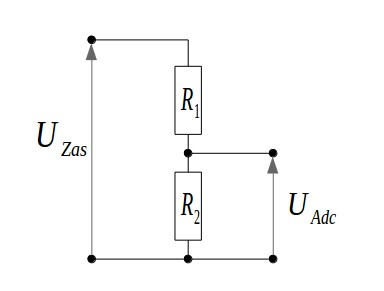
\includegraphics[scale=0.4]{dzielnikNapiecia.jpg}
    \caption{Dzielnik napięcia układu pomiarowego poziomu napięcia pakietu zasilającego.}
    \label{fig:równia}
\end{figure}

Napięcie na wyjściu dzielnika napięcia określone jest zależnością:
\begin{equation}
    U_{Adc}=U_{Zas}\frac{R_2}{R_1 + R_2}
    \label{eq:rownanieDzielnik}
\end{equation}

Zakładając maksymalną wartość napięcia pakietu, napięcie wejściowe na przetworniku analogowo-cyfrowym powinno wynosić 3.3V a rezystancja $R_2$ jest równa 10k$\Omega$, to zgodnie z zależnością (\ref{eq:rownanieDzielnik}) rezystancja $R_1$ powinna przyjąć około 15k$\Omega$.

Przetwornik analogowo-cyfrowy przetwarza sygnał analogowy na równoważną postać cyfrową. Mikrokontroler wyposażony jest w przetwornik 12-bitowy. Oznacza to, że do reprezentacji całego zakresu pomiarowego używa dwunastu bitów. Zakres pomiarowy określony jest przez sygnały referencyjne - 0V i 3.3V \cite{tiva}. Wartość zwracana przez przetwornik dla napięcia 0V wynosi 0, natomiast dla napięcia 3.3V jest równa 4096. Rozdzielczość przetwornika wynosi około 0.8mV

Zgodnie z pkt. \ref{niskiPoziom}, zgłaszane są dwa stany alarmowe związane z zasilaniem:
\begin{itemize}
\item
    stan niskiego poziomu naładowania pakietu zasilającego, gdy napięcie na akumulatorze jest mniejsze bądź równe 6.8V,
\item
    stan rozładowania pakietu zasilającego, gdy napięcie na akumulatorze jest mniejsze bądź równe 6V.
\end{itemize}

Biorąc pod uwagę powyższe zależności i założenia, można wyznaczyć wartości zwracane przez przetwornik dla stanów alarmowych, które przedsatwiono w tabeli \ref{tab:napieciaDwojnik}

\begin{table}[h]
    \caption{Poziomy napięć alarmowych oraz wartości zwracane przez przetwornik:}
    \begin{center}
		\label{tab:napieciaDwojnik}
		\begin{tabular}{|c|c|c|}
			\hline
 			\textbf{Napięcie $U_{Zas}$ [V]}& \textbf{Napięcie $U_{Adc}$ [V]}& \textbf{Wartość zwracana przez przetwornik} \\
 			\hline
 			6.8 & 2.72 & 3376 \\  
 			\hline
			6.0 & 2.4 & 2979 \\
			\hline
		\end{tabular}
	\end{center}
\end{table}

Pomiar poziomu napięcia dokonywany jest w trakcie zadania cyklicznego, wyzwalanego przez układ czasowo-licznikowy z częstotliwością 1Hz.




